\section{Proposed approach}
\label{sec:apprach}

Given a set of existing DSLs (that we term as the \textit{input set}) our approach is intended to identify commonalities --and so, potential reuse--. Then, we provide some metrics that permit to objectively evaluate those commonalities. The reminder of this section explain how we tackle this problem.

\subsection{Identifying commonalities}
\label{sec:metrics}

In the first part of our approach, we perform static analysis in syntax and semantics of a given set of DSLs in order to build a pair of Venn diagrams that allows language designers to easily visually identify commonalities among DSLs under study. The idea is to visualize each DSL as a pair of two sets: The first one is a set of metaclasses representing the syntax, and the second one is a set of domain-specific actions representing the semantics. Syntactic and semantic commonalities are represented as intersections between the corresponding sets. To this end, we designed an algorithm that is able to compute the all intersections among the syntax of the DSLs in the input set. 

Our algorithm for detecting \textbf{syntactic intersections} can be described as by the function that receives a set of metamodels (one for each DSL of the input set) and returns a set of tuples containing all the intersections among these metamodels. Note that there can be intersections among any of the combinations of the input set. Hence, in the result there is a tuple for each of the possible combinations of the input metamodels (i.e., the power set). Similarly, our algorithm for detecting \textbf{semantic intersections} can be described as a function that receives a set of aspects (one for each DSL of the input set) and returns a set of tuples containing all the intersections among these aspects. 

%\begin{equation}
%  Venn_{syn} : set(MM) \rightarrow set(<set(MM),set(MC)>)
%\end{equation}

%\begin{equation}
%  Venn_{syn}(mms) = \{<x,y> \mid x \in \mathcal{P}(mms), y = I_{syn}(x)\}
%\end{equation}

%Note that our algorithm relies on a function $I_{syn}$ that computes the intersection existing withing a given set of metamodels. It can be formalized as follows:

%\begin{equation}
%  I_{syn} : set(MM) \rightarrow set(MC)
%\end{equation}
%\vspace{-2mm}
%\begin{equation}
%  I_{syn}(mms) = \bigcap _{i=0}^{|mms|}mms_i
%\end{equation}

%Similarly, our algorithm for detecting \textbf{semantic intersections} can be described as a function that receives a set of aspects (one for each DSL of the input set) and returns a set of tuples containing all the intersections among these aspects. 

%\begin{equation}
%  Venn_{sem} : set(A) \rightarrow set(<set(A),set(DSA)>)
%\end{equation}

%\begin{equation}
%  Venn_{syn}(mms) = \{<x,y> \mid x \in \mathcal{P}(mms), y = I_{sem}(x)\}
%\end{equation}
%\vspace{2mm}

%This time, the algorithm for semantic commonalities relies on a function $I_{sem}$ that computes the intersection existing withing a given set of aspects. It can be formalized as follows:

%\begin{equation}
%  I_{sem} : set(A) \rightarrow set(DSA)
%\end{equation}
%\vspace{-2mm}
%\begin{equation}
%  I_{sem}(dsas) = \bigcap _{i=0}^{|dsas|}dsas_i
%\end{equation}

\subsubsection{Comparison operators:} A syntactic intersection is a set of metaclasses that are equal in two or more DSLs. Similarly, a semantic intersection is a set of domain-specific actions that are equal in two or more DSLs. At this point we need to clearly define the notion of equality between metaclasses and domain-specific actions. That is, we need to establish the criteria under we consider that two metaclasses/domain-specific actions are equal.

\begin{itemize}
\item \textbf{Comparison of metaclasses:} The name of a metaclass usually corresponds to a word that evokes the domain concept the metaclass represents. Thus, intuitively one can think that a first approach to compare meta-classes is by comparing their names. As we will see later in this paper, this approach results quite useful and it is quite probable that, we can find potential reuse.

%\begin{equation}
%  \doteq~: MC \times MC \rightarrow bool
%\end{equation}
%\vspace{-1mm}
\begin{equation}
\begin{split}
  MC_{A} \doteq MC_{B} &= true \implies \\
   & MC_{A}.name = MC_{B}.name
 \end{split}
\end{equation}

\vspace{1mm}
\hspace{3mm} Unfortunately, comparison of metaclasses by using only their names might have some problems. There are cases in which two meta-classes with the same name are not exactly the same since they do not represent the same domain concept or because there are domains that use similar vocabulary. In such cases, an approach that certainly helps is to compare meta-classes not only by their names but also by their attributes and references. Hence, we define a second comparison operator for metaclasses i.e., $\doteqdot $.

%\begin{equation}
%  \doteqdot~: MC \times MC \rightarrow bool
%\end{equation}
%\vspace{-1mm}
\begin{equation}
\begin{split}
  MC_{A} \doteqdot MC_{B} &= true \implies \\
   & MC_{A} \doteq = MC_{B} ~ \wedge \\
   & \forall a_1 \in MC_{A}.attr \mid (\exists a_2 \in MC_{B}.attr \mid a_1 = a_2) ~ \wedge \\
   & \forall r_1 \in MC_{A}.refs \mid (\exists r_2 \in MC_{B}.refs \mid r_1 = r_2)
  \end{split}
\end{equation}

\vspace{2mm}
\hspace{3mm} Although this second approach might be too restrictive, it implies that the specification of the two meta-classes are exactly the same so potential reuse is guaranteed. At the implementation we provide support for the two comparison approaches explained above. However, additional comparison operators such as the surveyed in \cite{Lafi:2011} can be easily incorporated.

\vspace{2mm}

\item \textbf{Comparing domain-specific actions:} Like methods in Java, domain-specific actions have a signature that specifies its contract (i.e., return type, visibility, parameters, name, and so on), and a body where the behavior is actually implemented. In that sense, the comparison of two domain-specific actions can be performed by checking if their signatures are equal. This approach is practical and also reflects potential reuse; one might think that the probability that two domain-specific actions with the same signatures are the same is elevated.

%\begin{equation}
%  \circeq~: DSA \times DSA \rightarrow bool
%\end{equation}
%\vspace{-1mm}
\begin{equation}
\begin{split}
  DSA_{A} & \circeq DSA_{B} = true \implies \\
   & DSA_{A}.name = DSA_{B}.name ~ \wedge \\
   & DSA_{A}.returnType = DSA_{B}.returnType ~ \wedge \\
   & DSA_{A}.visibility = DSA_{B}.visibility ~ \wedge \\
   & \forall p_1 \in DSA_{A}.params \mid (\exists p_2 \in DSA_{B}.params \mid p_1 = p_2)
 \end{split}
\end{equation}

\vspace{2mm}
\hspace{3mm} However, as the reader might imagine, there are cases in which signatures comparison is not enough. Two domain-specific actions defined in different DSLs can perform different computations even if they have the same signatures. As a result, a second approach relies in the comparison of the bodies of the domain-specific actions. Note that such comparison can be arbitrary difficult. Indeed, if we try to compare  the behavior of the actions we will have to deal with the semantic equivalence problem that, indeed, is known as be undecidable \cite{Lucanu:2013}. In this case, we a conservative approach is to compare only the structure (abstract syntax tree) body of the domain-specific action. To this end, we use the API for java code comparison proposed in \cite{Biegel:2010}. 

%\begin{equation}
%  \triangleq~: DSA \times DSA \rightarrow bool
%\end{equation}
%\vspace{-1mm}
\begin{equation}
\begin{split}
  DSA_{A} \triangleq DSA_{B} & = true \implies \\
   & DSA_{A} \circeq DSA_{B} ~ \wedge \\
   & DSA_{A}.AST = DSA_{B}.AST
 \end{split}
\end{equation}
\end{itemize}


%It is worth nothing that there is this phenomenon of \textit{semantical variability}. A necessary condition to decide whether two language constructs are equivalent is that both, the metaclass and the associated domain-specific actions are equivalent. This condition guarantees that the specification is the same not only at the level of the abstract syntax but also at the level of the semantics. However, there is a phenomenon in the literature that corresponds to semantical variability \cite{Cengarle:2009}. There is semantical variability when there there are two constructs that have the same abstract syntax (i.e., their metaclasses are equal) but that differ in the domain-specific actions. This case is of interest for us because even in the presence of semantical variability we can have some potential reuse. If the metaclasses of two constructs are the same we can reuse them even if their domain-specific actions are different. 

\vspace{-2mm}
\subsubsection{Visualizing the results:} Figure \ref{fig:shape} shows the Venn Diagram for the case of our motivating scenario. In that figure we can see that the family is an overlapping family in terms of the abstract syntax. In the case of the semantics the results are quite interesting. Note that depending on the type of comparison operator we have different results. When the comparison operator is the naming, we have the same overlapping shape that in the case of the abstract syntax. However, when the operators become more restrictive the overlapping region is reduced. 

\begin{figure}
\centering
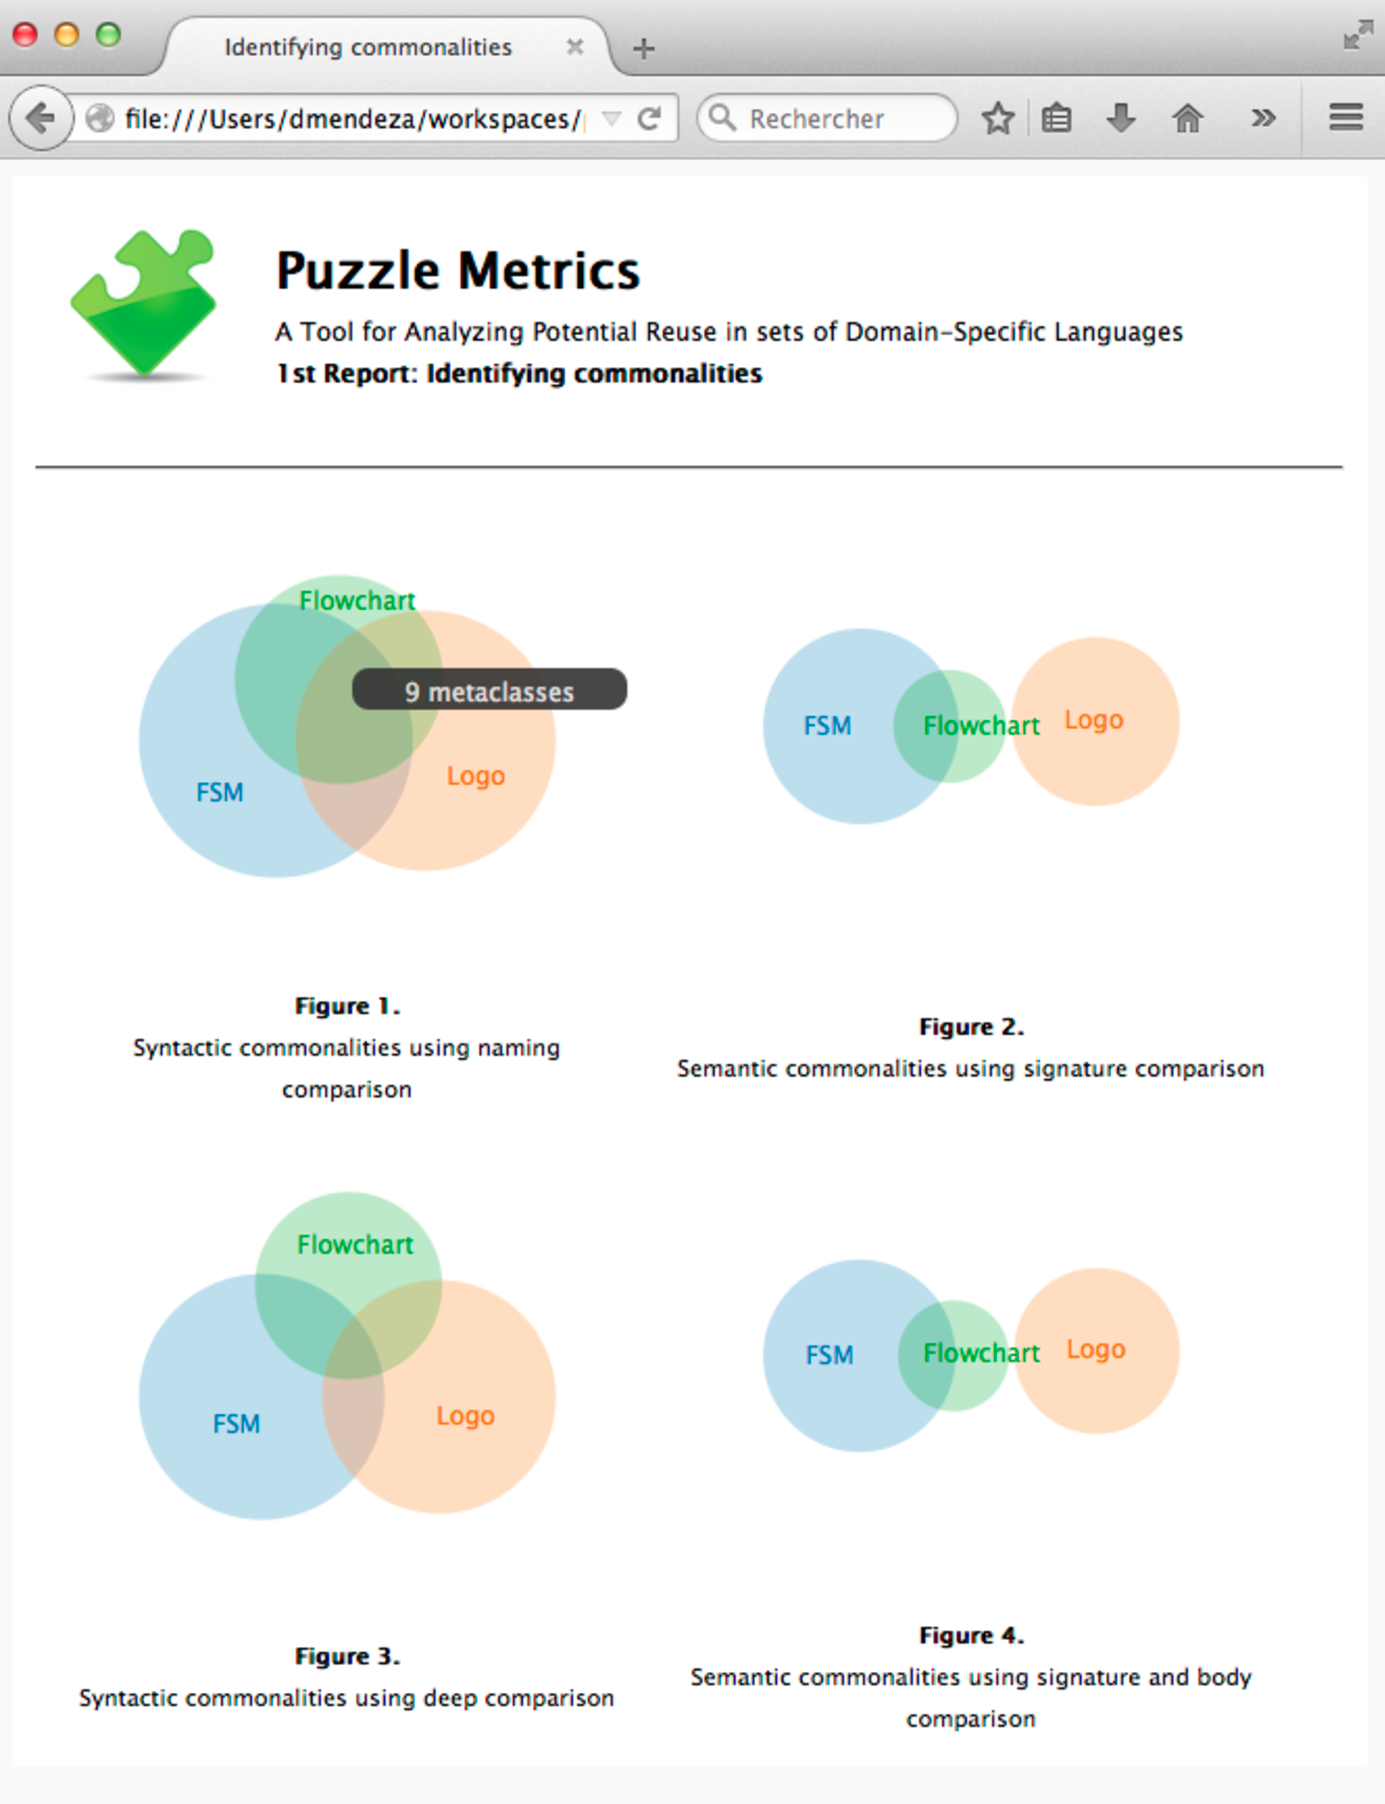
\includegraphics[width=1\linewidth]{images/domains-inaction.pdf}
\caption{Visualizing syntactic and semantic commonalities}
\label{fig:shape}
\end{figure}

%\vspace{-2mm}
%\subsubsection{Visualizing semantical variability:} Note that the phenomenon of semantical variability is evident in the example presented. Where there are syntactic commonalities between DSLs Logo and FSM, there are not semantic commonalities. As an additional feature of our approach, we provide a visualization of the semantical variability phenomenon. The idea is that language designers can see what are the variations in the domain specific actions.

\subsection{Extracting reusable language modules}

After being identifying commonalities among the input set, we extract a set of reusable language modules. The idea is to be able to extract set of DSLs that are used by different DSLs. Our partitioning strategy can be graphically summarized in Figure X. We propose to break down the set of DSLs by extracting the intersections in the Venn diagram. 

\subsubsection{Breaking down the input set}

Figure \ref{fig:breakingdown} shows the way in which we break down the input set. 

\begin{figure}
\centering
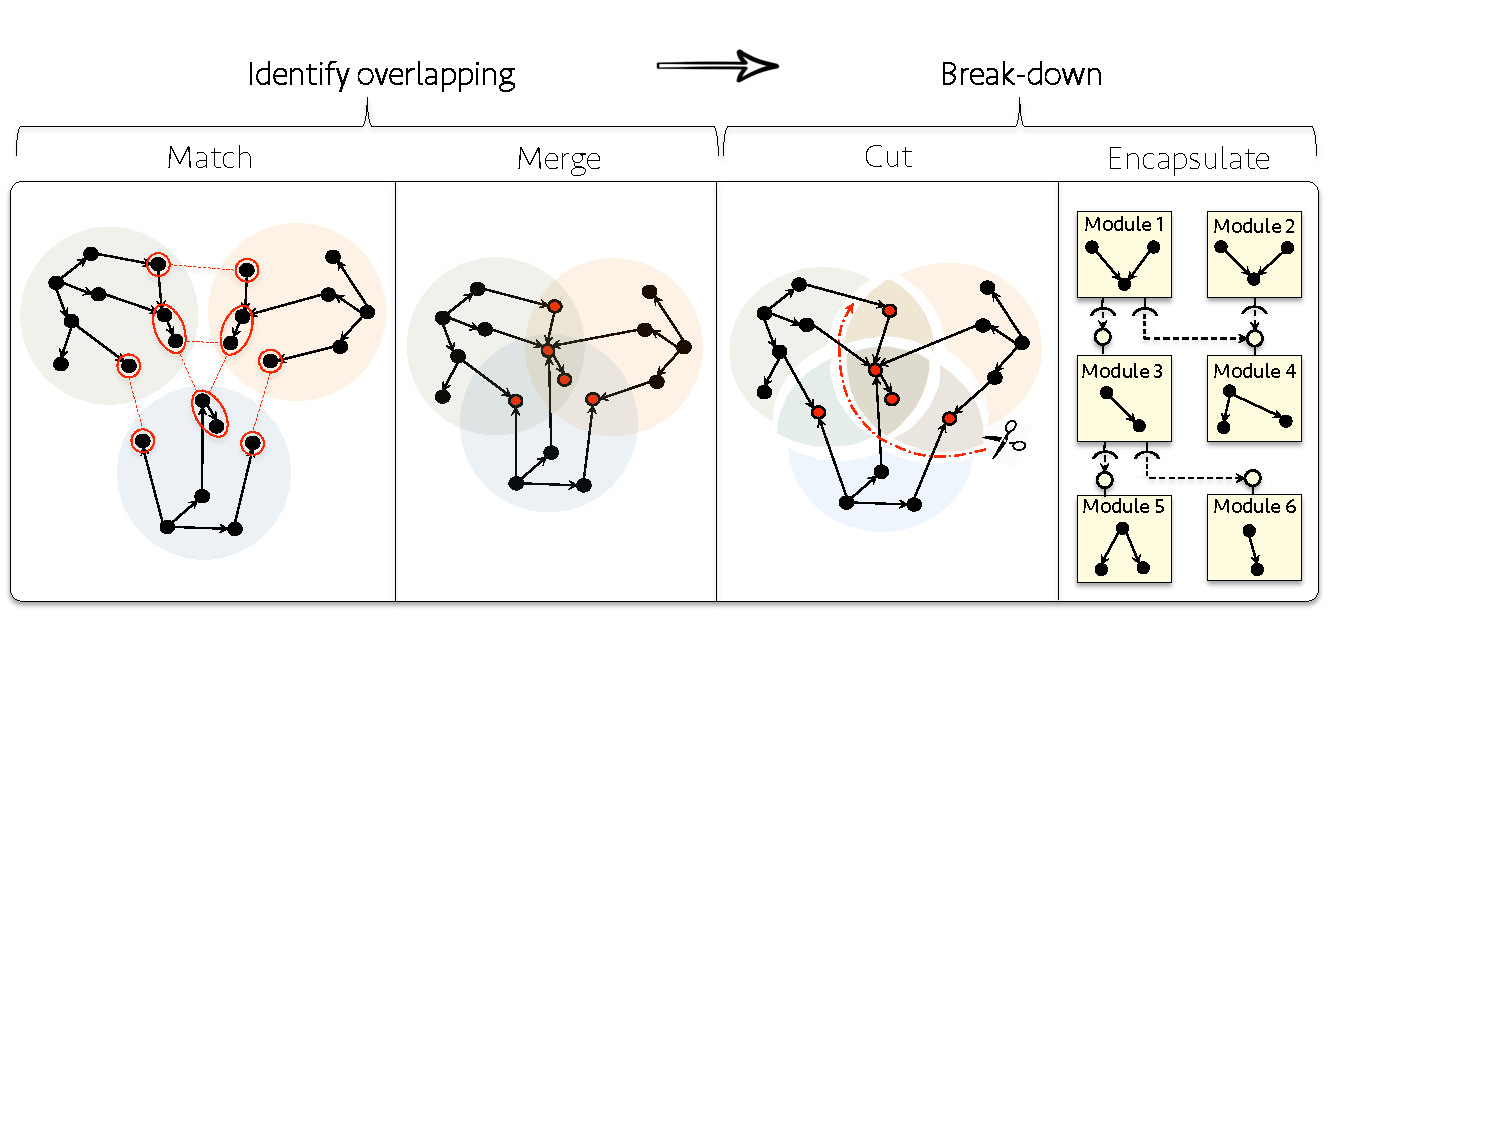
\includegraphics[width=1.05\linewidth]{images/breakdown.pdf}
\caption{Breaking down the input set by separating intersections}
\label{fig:breakingdown}
\end{figure}

\subsubsection{Modularization support}

\subsection{Composing reusable language modules}

It is important to highlight that our approach is useful only if the extracted language modules can be later composed to obtain new DSLs. In this section we present our composition approach that shows how this composition is supported. 
